\documentclass[conference]{IEEEtran}
\IEEEoverridecommandlockouts
% The preceding line is only needed to identify funding in the first footnote. If that is unneeded, please comment it out.
\usepackage{cite}
\usepackage{amsmath,amssymb,amsfonts}
\usepackage{graphicx}
\usepackage{textcomp}
\usepackage{xcolor}
\def\BibTeX{{\rm B\kern-.05em{\sc i\kern-.025em b}\kern-.08em
    T\kern-.1667em\lower.7ex\hbox{E}\kern-.125emX}}
\title{
\vspace{1cm}
{
\includegraphics[width=0.15\textwidth]{ /storage/emulated/0/vignan/IMG-20241018-WA0001.jpg} \\ Platformio Assignment}}
\author{Bynaboyina Aiswarya \\ Roll No: FWC22295 \\ aiswaryabaiswarya61@gmail.com}
 \begin{document}
\maketitle
 \section{ABSTRACT}

This paper presents the design and realizatio    n of a four-variable Boolean function using two cascaded $4 \times 1$ multiplexers. The multiplexers take inputs \( U, V, W, X \) and output the minimized Boolean function \( F(U, V, W, X)\).                                       The system uses standard logic principles to     reduce complexity and efficiently compute the     Boolean expression. This implementation is aimed at providing a compact, reliable solution for logic circuit design, suitable for educational and industrial applications where Boolean minimization and multiplexer-based designs are needed.

\begin{figure}[h]                          
	\centering
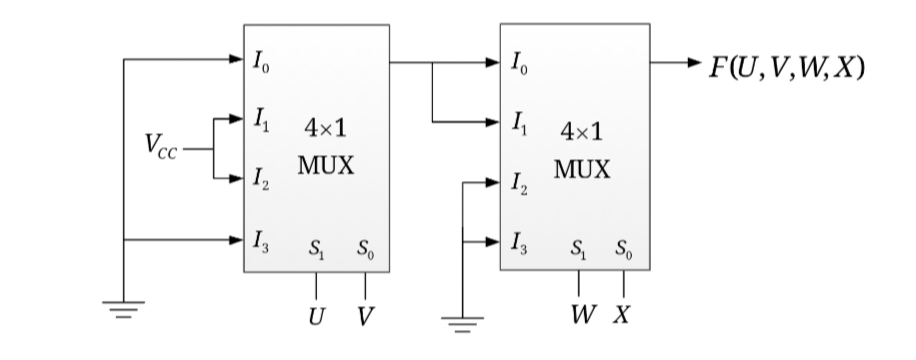
\includegraphics[width=0.3\textwidth]{  /storage/emulated/0/vignan/IMG_20241019_122635.jpg }
\caption{\label{fig:Gates}}                
\end{figure}


\subsection{Truth Table for $4 \times 1$ mux}

\begin{table}[htbp]
    \centering
\begin{tabular}
{ | c | c | c | c | c | c | } \hline
$U$ & $V$ & $W$ & $X$ & $F_0$ & $F_1$ \\\hline
0   & 0   & 0   & 0   & 0     & 0 \\
0   & 0   & 0   & 1   & 0     & 0 \\
0   & 0   & 1   & 0   & 0     & 0 \\
0   & 0   & 1   & 1   & 0     & 0 \\
0   & 1   & 0   & 0   & 1     & 1 \\               
0   & 1   & 0   & 1   & 1     & 1 \\
0   & 1   & 1   & 0   & 1     & 0 \\               
0   & 1   & 1   & 1   & 1     & 0 \\
1   & 0   & 0   & 0   & 1     & 1 \\               
1   & 0   & 0   & 1   & 1     & 1 \\
1   & 0   & 1   & 0   & 1     & 0 \\               
1   & 0   & 1   & 1   & 1     & 0 \\               
1   & 1   & 0   & 0   & 0     & 0 \\               
1   & 1   & 0   & 1   & 0     & 0 \\               
1   & 1   & 1   & 0   & 0     & 0 \\               
1   & 1   & 1   & 1   & 0     & 0  \\ \hline
\end{tabular}
\vspace{0.15cm}
\caption{\label{tab:widgets}}
\end{table}
					     This truth table shows all input combinationsfor a $4\times1$ multiplexer. It lists corresponding outputs based on input conditions.


\section{COMPONENTS} 

\begin{figure}[h]                           
\centering                           
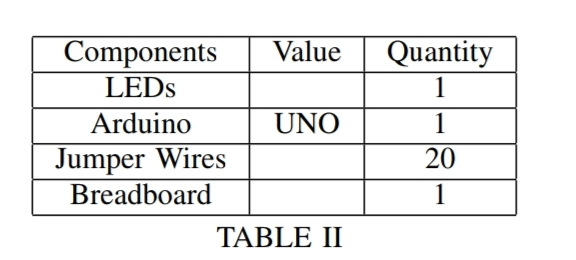
\includegraphics[width=0.3\textwidth] {/storage/emulated/0/vignan/IMG_20241018_171312.jpg}            
\end{figure}

\section{PROCEDURE}
 \begin{enumerate}
\item Connect the led to the arduino uno.
\item Give the inputs manually using jumper wires.
\item Check the outputs by chaning inputs as per truth table of the $4 \times 1$ mux.
\item Execute the arduino code using the pio run command in nvim editor.
\item After upload the code into hardware setup using arduino IDE platform.
 \end{enumerate}

\section{RESULTS}
 \begin{enumerate}
\item Download the codes given in the link below and execute them to see the output as shown in figure 2.
\item https://github.com/BynaboyinaAiswarya/Fwc-/blob/main/Platformio/main.cpp
 \end{enumerate}
\section{CONCLUSION}
In the below figure we can see the hardware connection between arduino uno and led using jumper wires in bread board and by giving manual inputs in bread board we can observe the outputs of truth tables in terms of led. 
\begin{figure}[h] 
	\centering 
	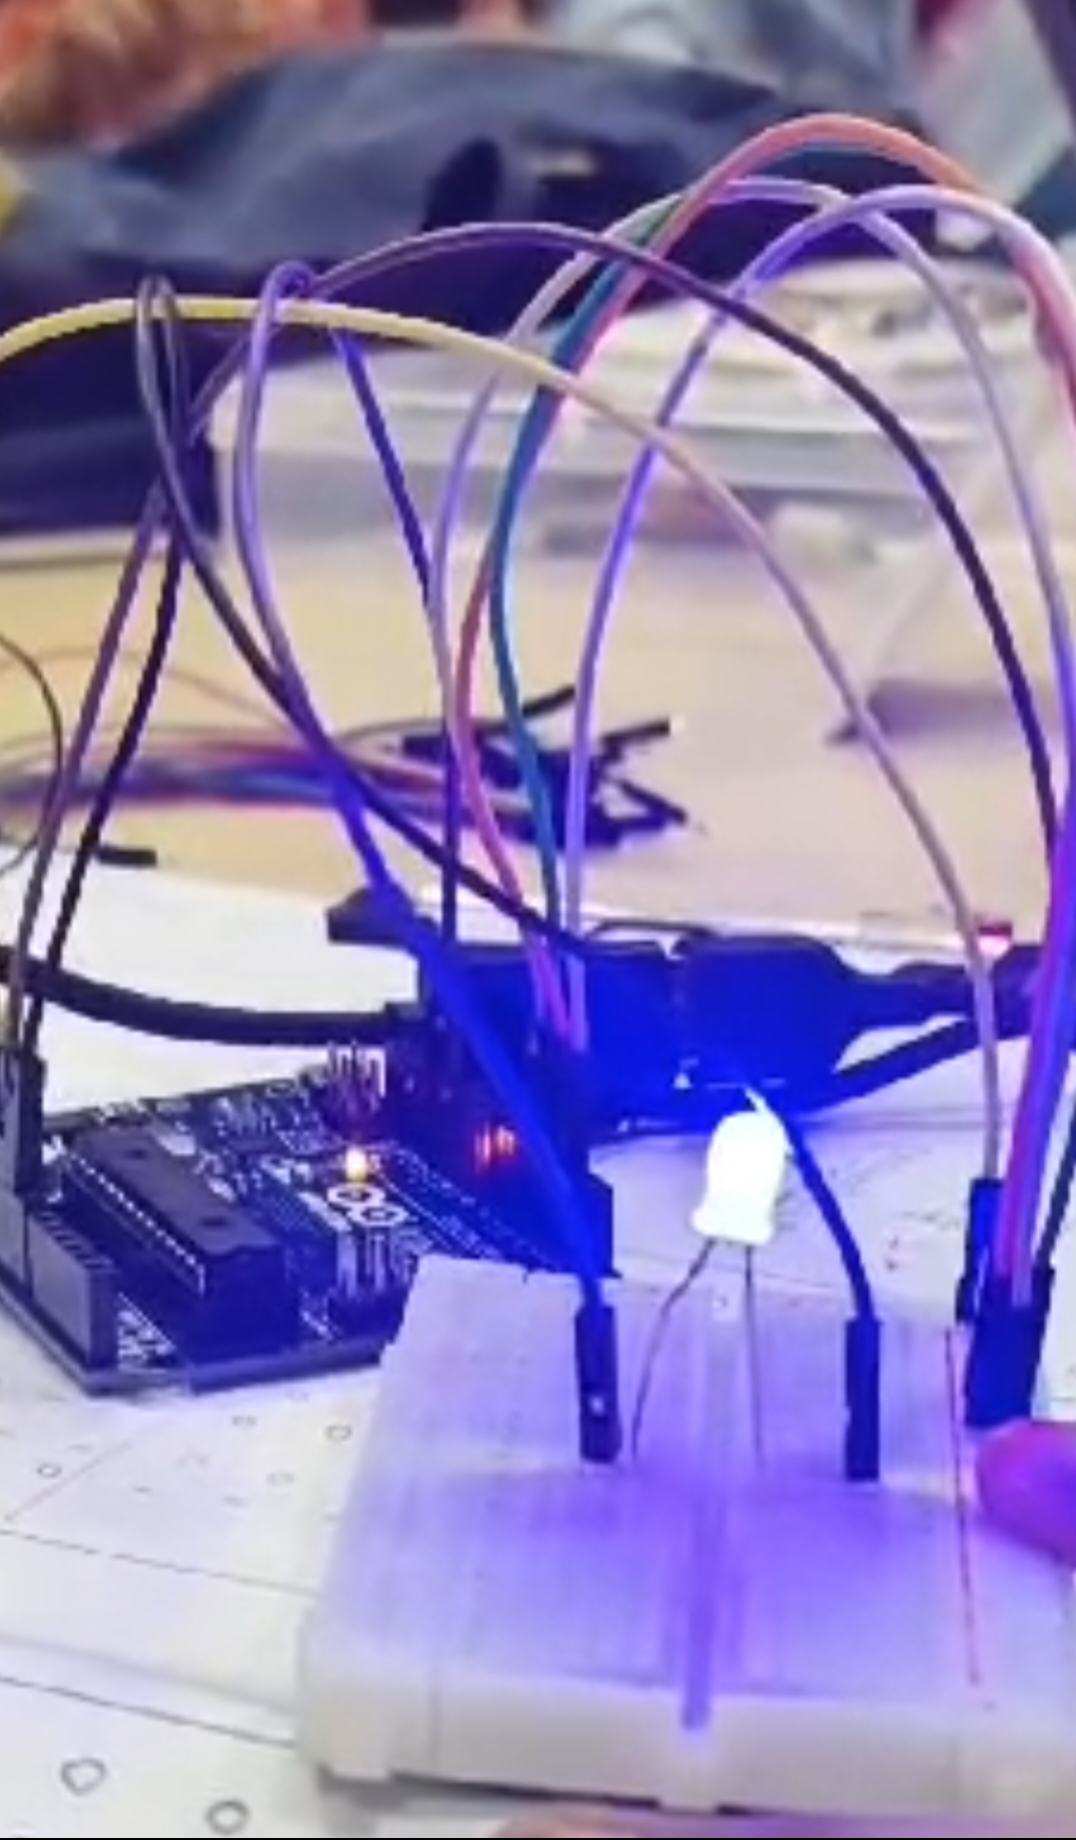
\includegraphics[width=0.3\textwidth]{ /storage/emulated/0/vignan/IMG_20241018_164936.jpg }
	\caption{\label{fig:Gates}}    
\end{figure}
Hence implementation of $4 \times 1$ mux using led is done and verified through truth table of $4 \times 1$.


\end{document}
